% Beamer Presentation
% LaTeX Template
% Version 1.0 (10/11/12)
%
% This template has been downloaded from:
% http://www.LaTeXTemplates.com
%
% License:
% CC BY-NC-SA 3.0 (http://creativecommons.org/licenses/by-nc-sa/3.0/)
%
%%%%%%%%%%%%%%%%%%%%%%%%%%%%%%%%%%%%%%%%%

%----------------------------------------------------------------------------------------
%   PACKAGES AND THEMES
%----------------------------------------------------------------------------------------


    \documentclass[xcolor=dvipsnames]{beamer}

    \mode<presentation> {

    % The Beamer class comes with a number of default slide themes
    % which change the colors and layouts of slides. Below this is a list
    % of all the themes, uncomment each in turn to see what they look like.


    \usetheme[width=1.55cm, height=2cm]{PaloAlto}

    % As well as themes, the Beamer class has a number of color themes
    % for any slide theme. Uncomment each of these in turn to see how it
    % changes the colors of your current slide theme.

    \usecolortheme{dove}


    %\setbeamertemplate{footline} % To remove the footer line in all slides uncomment this line
    %\setbeamertemplate{footline}[page number] % To replace the footer line in all slides with a simple slide count uncomment this line

    %\setbeamertemplate{navigation symbols}{} % To remove the navigation symbols from the bottom of all slides uncomment this line
    }

    \usepackage[spanish]{babel}
    \usepackage[utf8]{inputenc}

    \usepackage{graphicx} % Allows including images
    \usepackage{booktabs} % Allows the use of \toprule, \midrule and \bottomrule in tables
    \usepackage{multimedia}
    \usepackage{geometry}
    \usepackage{wrapfig}
    \usepackage{multicol}
    \usepackage{vwcol}
    \usepackage{anyfontsize}
    \usepackage[export]{adjustbox}

    %\usepackage{titlesec} % Allows customization of titles
    %\usepackage{pdfpages}
    \usepackage{multirow}
    \usepackage{array}

    %\setbeamertemplate{frametitle}[center]
    
    \definecolor{Ines}{RGB}{255,20,147}
    \definecolor{Jaime}{RGB}{255,165,0}
    \definecolor{Jaime1}{RGB}{255,195,100}
    \usefonttheme{serif}
    

    \setbeamercolor{frametitle}{bg=Jaime1}
    \setbeamercolor{frametitle}{fg=Orchid}
    \setbeamercolor{logo}{bg=gray}
    \setbeamercolor{sidebar}{bg=Jaime1}
    \setbeamercolor{section in sidebar}{fg=Orchid} 
    \setbeamercolor{section in sidebar shaded}{fg=Orchid}
    \setbeamercolor{title in sidebar}{fg=Orchid}
    \setbeamercolor{author in slidebar}{fg=black}

%----------------------------------------------------------------------------------------
%   TITLE PAGE
%----------------------------------------------------------------------------------------

    \title[\textbf{MuDeb}]{Red de Difusión de Física de Partículas} % The short title appears at the bottom of every slide, the full title is only on the title page

    \author[]{Jaime Díez González-Pardo } % Your name

    \institute[UC]{Universidad de Cantabria}

    \date{ \today} % Date, can be changed to a custom date
    \newif\ifplacelogo % create a new conditional
    \placelogotrue % set it to true
    \logo{
\includegraphics[scale=0.06]{../Fotos/Logo/logoFinal.png}}

%----------------------------------------------------------------------------------------
%   Main Document
%----------------------------------------------------------------------------------------

    \begin{document}

        \begingroup
            \makeatletter
            \setlength{\hoffset}{-.5\beamer@sidebarwidth}
            \makeatother
            \begin{frame}[plain]
                    \vspace{1cm}
                    \begin{center}
                       {\fontsize{35pt}{24pt}\selectfont {\color{Jaime} \textbf{R}}ed de {\color{Orchid} \textbf{D}}ifusión de {\color{Jaime} \textbf {F}}ísica de {\color{Orchid} \textbf{P}}artículas}
                    \end{center}
                    \vspace{1cm}

                \begin{columns}[onlytextwidth,T]
                    \column{\dimexpr\linewidth-35mm}%-5mm}
                        
                        \normalsize
                        \vspace{0.75cm}
                            \insertauthor
                        \vspace{1cm}

                        \insertinstitute

                        \insertdate

                    \column{35mm}
                        
\includegraphics[width=35mm]{../Fotos/Logo/logoTrans.png}

                \end{columns}
            \end{frame}
        \endgroup

            \section{Fisica Tendencia}
                % Tendencia
                \begin{frame}
                    \frametitle{\centerline{\textbf{La Física está de Moda}}}
                    \onslide<1->{
                    %\vspace{-4cm}
                    \begin{minipage}[c]{0.25\linewidth}
                        \begin{figure}[b]
                            \centering
                            
\includegraphics[scale=0.35]{Fotos/Carreras/MasPujantes.png}
                        \end{figure}
                        
                    \end{minipage}}
                    \onslide<2->{\begin{minipage}[c]{0.3\linewidth}
                        \vspace{0.7cm}
                        \begin{figure}[t]
                            \centering
                            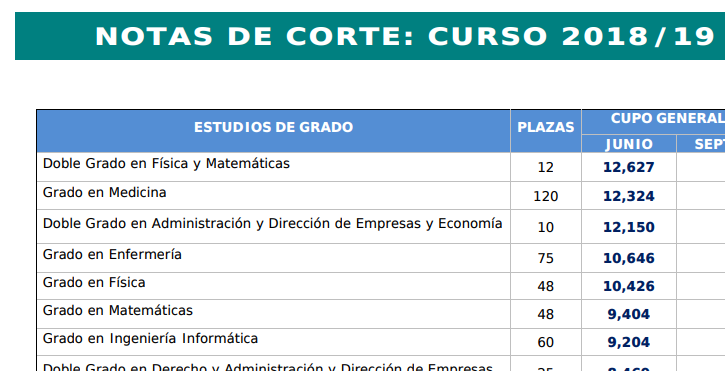
\includegraphics[scale=0.3]{Fotos/Carreras/notaCorte.png}
                        \end{figure}
                        
                    \end{minipage}
                    }

                    \vspace{-3cm}

                    \onslide<3->{\begin{minipage}[c]{1\linewidth}
                        \begin{figure}[H]
                            \centering
                            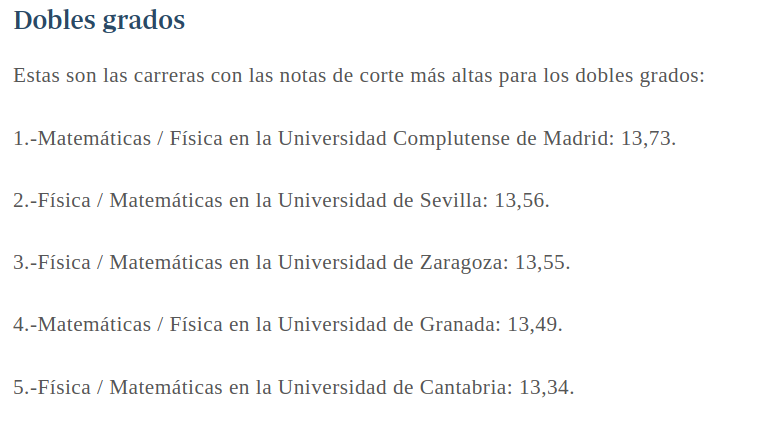
\includegraphics[scale=0.35]{Fotos/Carreras/DobleGrado.png}
                        \end{figure}
                    \end{minipage}}
                \end{frame}

                %motivos
                \begin{frame}
                    \frametitle{\centerline{\textbf{La Física está de Moda}}}
                    \onslide<1->{
                    %\vspace{-0.2cm}
                    \begin{minipage}[c]{0.3\linewidth}
                        \vspace{-2.2cm}
                        \begin{figure}[t]
                            \centering
                            
\includegraphics[scale=0.3]{Fotos/Motivos/Business.jpg}
                        \end{figure}
                    \end{minipage}}
                    \onslide<2->{\begin{minipage}[c]{0.6\linewidth}
                        \vspace{1.2cm}
                        \begin{figure}[b]
                            \centering
                            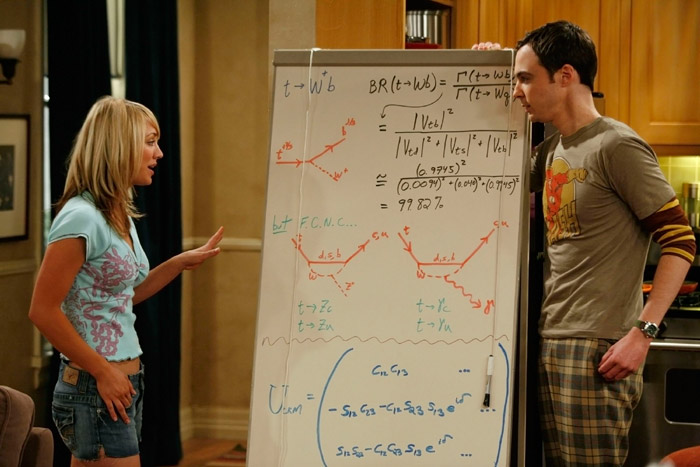
\includegraphics[scale=0.35]{Fotos/Motivos/bigbang.jpg}
                        \end{figure}
                        
                    \end{minipage}}
                \end{frame}

                %Divulgacion
                \begin{frame}
                    \frametitle{\centerline{\textbf{La Divulgación de la Física}}}
                    \onslide<1->{
                    \vspace{-3cm}
                    \begin{minipage}[c]{0.3\linewidth}
                        \begin{figure}[t]
                            \centering
                            
\includegraphics[scale=0.4]{Fotos/Divulgacion/masterclasses.png}
                        \end{figure}
                    \end{minipage}}
                    \onslide<2->{\begin{minipage}[c]{0.6\linewidth}
                        \vspace{3cm}
                        \begin{figure}[b]
                            \centering
                            
\includegraphics[scale=0.2]{Fotos/Divulgacion/icecube.jpeg}
                        \end{figure}
                    \end{minipage}}
                    \vspace{-2cm}
                    \onslide<3->{\begin{minipage}[c]{0.6\linewidth}
                        {\begin{figure}[t]
                            \centering
                            
\includegraphics[scale=0.38]{Fotos/Divulgacion/nocheInvestigadores.jpeg}
                        \end{figure}}
                    \end{minipage}}
                    %\vspace{-2cm}
                    \onslide<4->{\begin{minipage}[c]{0.3\linewidth}
                        {\begin{figure}[b]
                            \centering
                            
\includegraphics[scale=0.38]{Fotos/Divulgacion/Sabados.jpg}
                        \end{figure}}
                    \end{minipage}}
                \end{frame}

            \section{Area de Divulgación}
                %Divulgacion
                \begin{frame}
                    \frametitle{\centerline{\textbf{Experimentos educativos de Física}}}
                    \onslide<1->{En la Universidad de Cantabria, entre primero y tercero de carrera se realizan:

                        \begin{table}[H]
                            \centering
                            \begin{tabular}{c c}
                                Prácticas Totales & $\approx$ 70 \\
                                Prácticas de Partículas & 1 \\ 
                            \end{tabular}
                        \end{table}}
                        \vspace{-3cm}
                    
                    \onslide<2->{\begin{minipage}[c]{0.2\linewidth}
                            \vspace{3cm}
                            \begin{figure}[t]
                                \centering
                                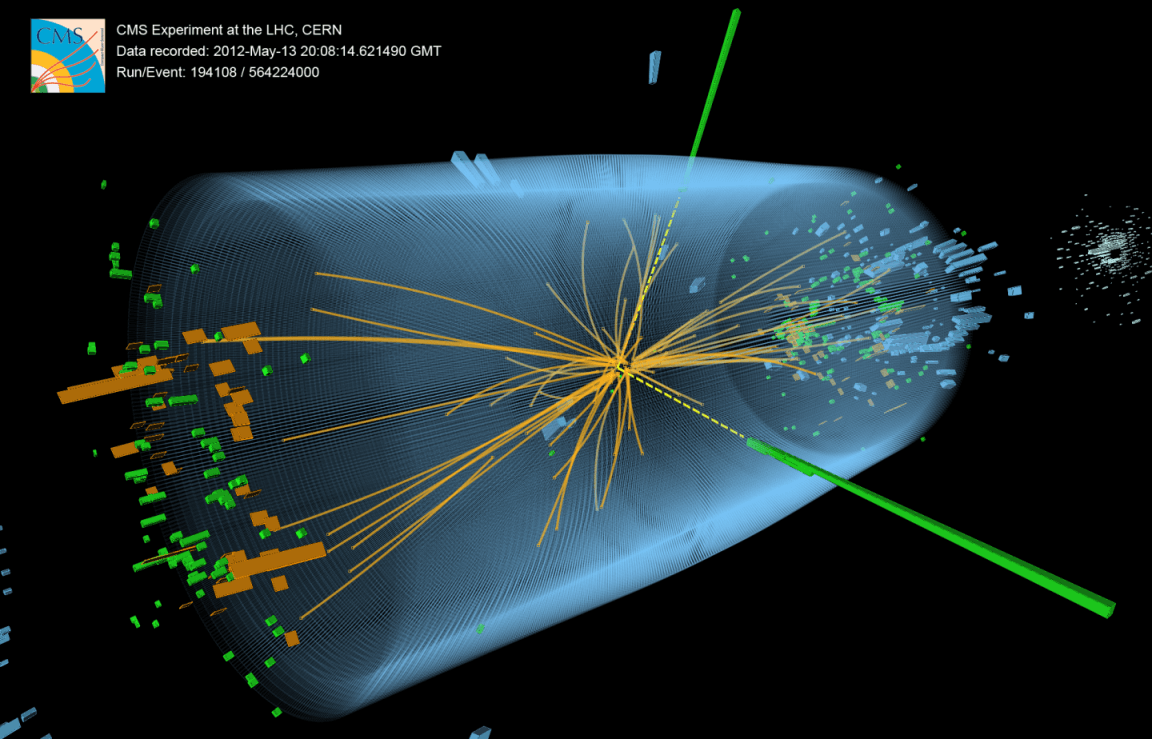
\includegraphics[scale=0.15]{Fotos/higgs-candidate.png}
                            \end{figure}
                        \end{minipage}}
                        \vspace{-3cm}

                    \onslide<3->{\begin{minipage}[c]{1.5\linewidth}
                        {\begin{figure}[b]
                            \centering
                            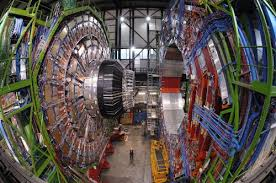
\includegraphics[scale=0.5]{Fotos/Divulgacion/CMS.jpeg}
                        \end{figure}}
                    \end{minipage}}
                \end{frame}

            \section{El Experimento}

                %Experimento
                \begin{frame}
                    \frametitle{\centerline{\textbf{Medida de la Vida Media del Muón}}}

                    \onslide<1->{%\begin{minipage}[c]{0.3\linewidth}
                        Experimento de la medida de la vida media del Muón a partir del tiempo de desintegración de muones cósmicos dentro del detector}
                    
                        \vspace{-3cm}
                    
                    \onslide<2->{\begin{minipage}[c]{1.4\linewidth}
                            \vspace{3cm}
                            \begin{figure}[t]
                                \centering
                                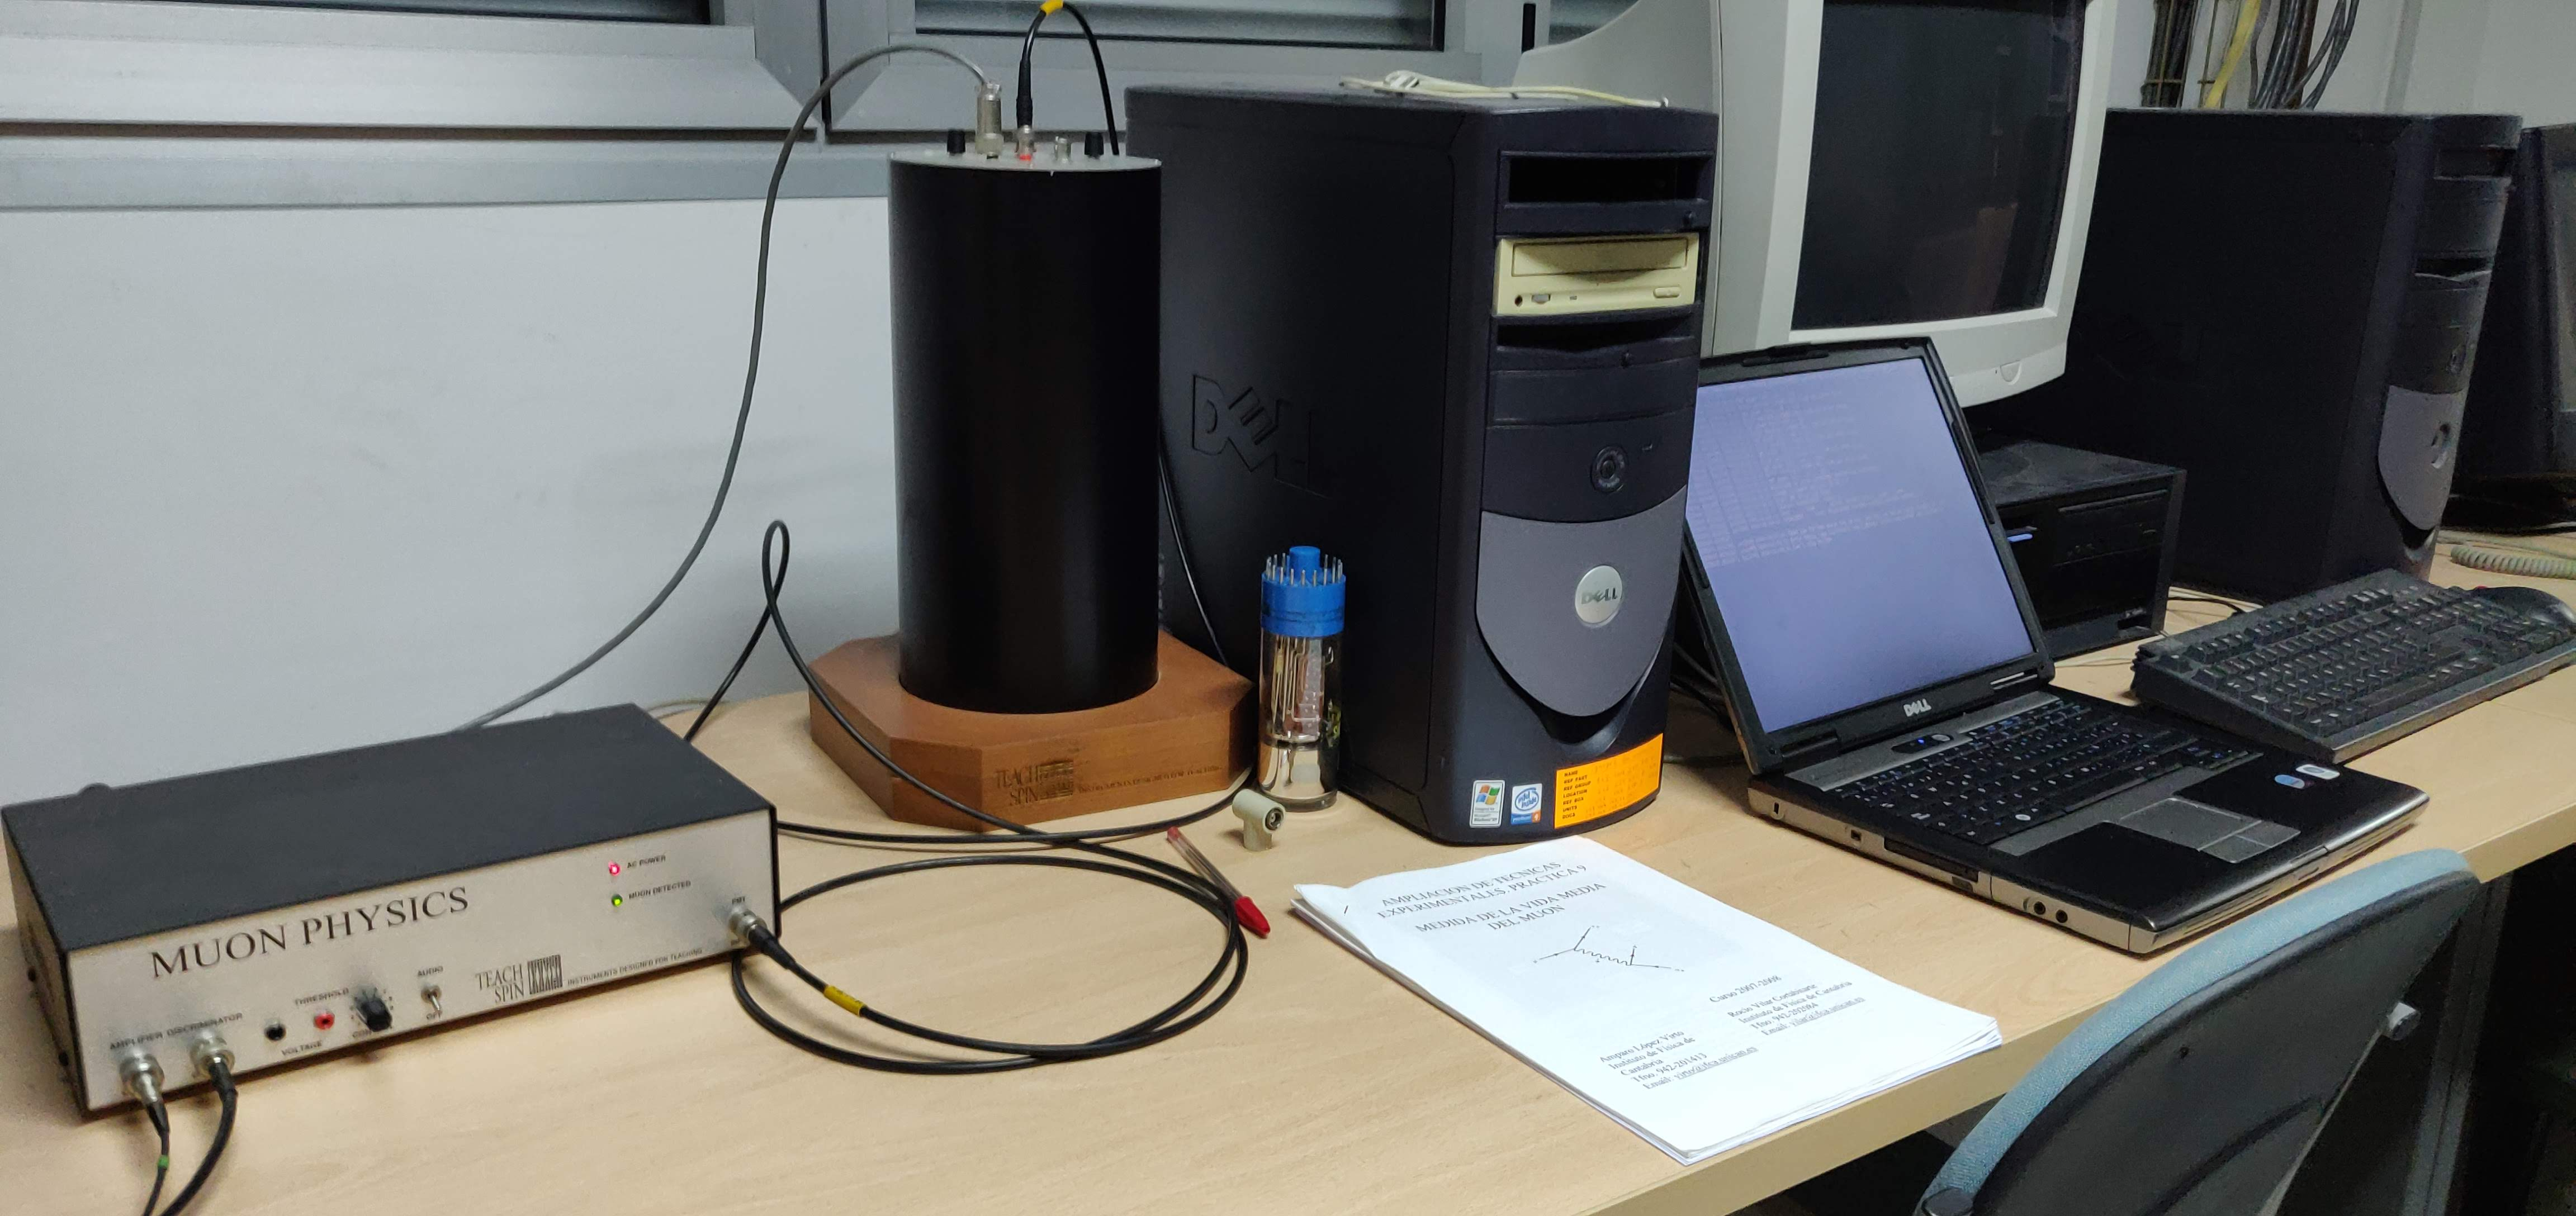
\includegraphics[scale=0.04]{Fotos/Experimento/IMG_20180927_113646.jpg}
                            \end{figure}
                        \end{minipage}}
                        \vspace{-1cm}

                    \onslide<3->{\begin{minipage}[c]{0.2\linewidth}
                        {\begin{figure}[b]
                            \centering
                            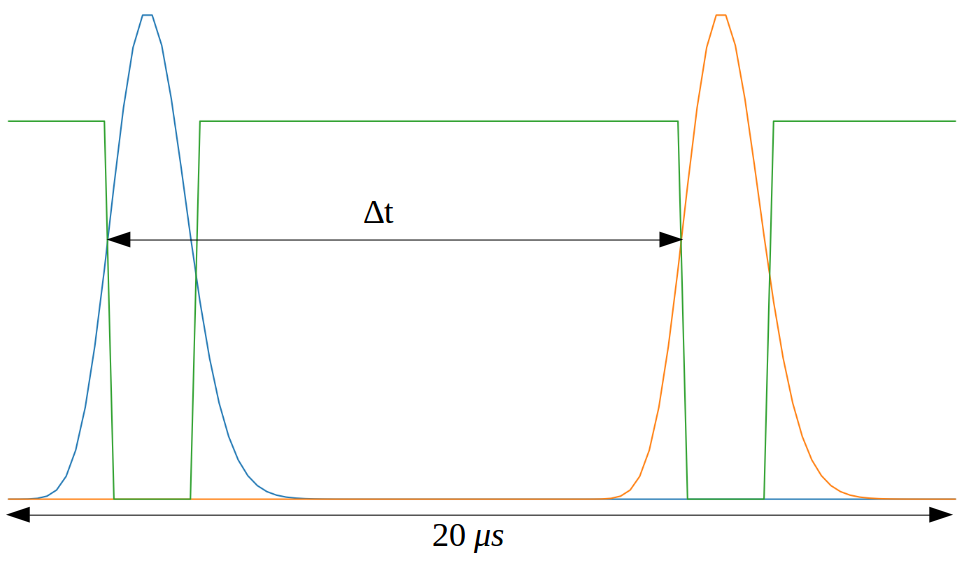
\includegraphics[scale=0.2]{Fotos/Experimento/signalLabels.png}
                        \end{figure}}
                    \end{minipage}}
                 \end{frame}

                 %Experimento
                \begin{frame}
                    \frametitle{\centerline{\textbf{Medida de la Vida Media del Muón}}}


                    \onslide<1->{\begin{minipage}[c]{0.2\linewidth}
                            \vspace{-0.3cm}
                            \begin{figure}[t]
                                \centering
                                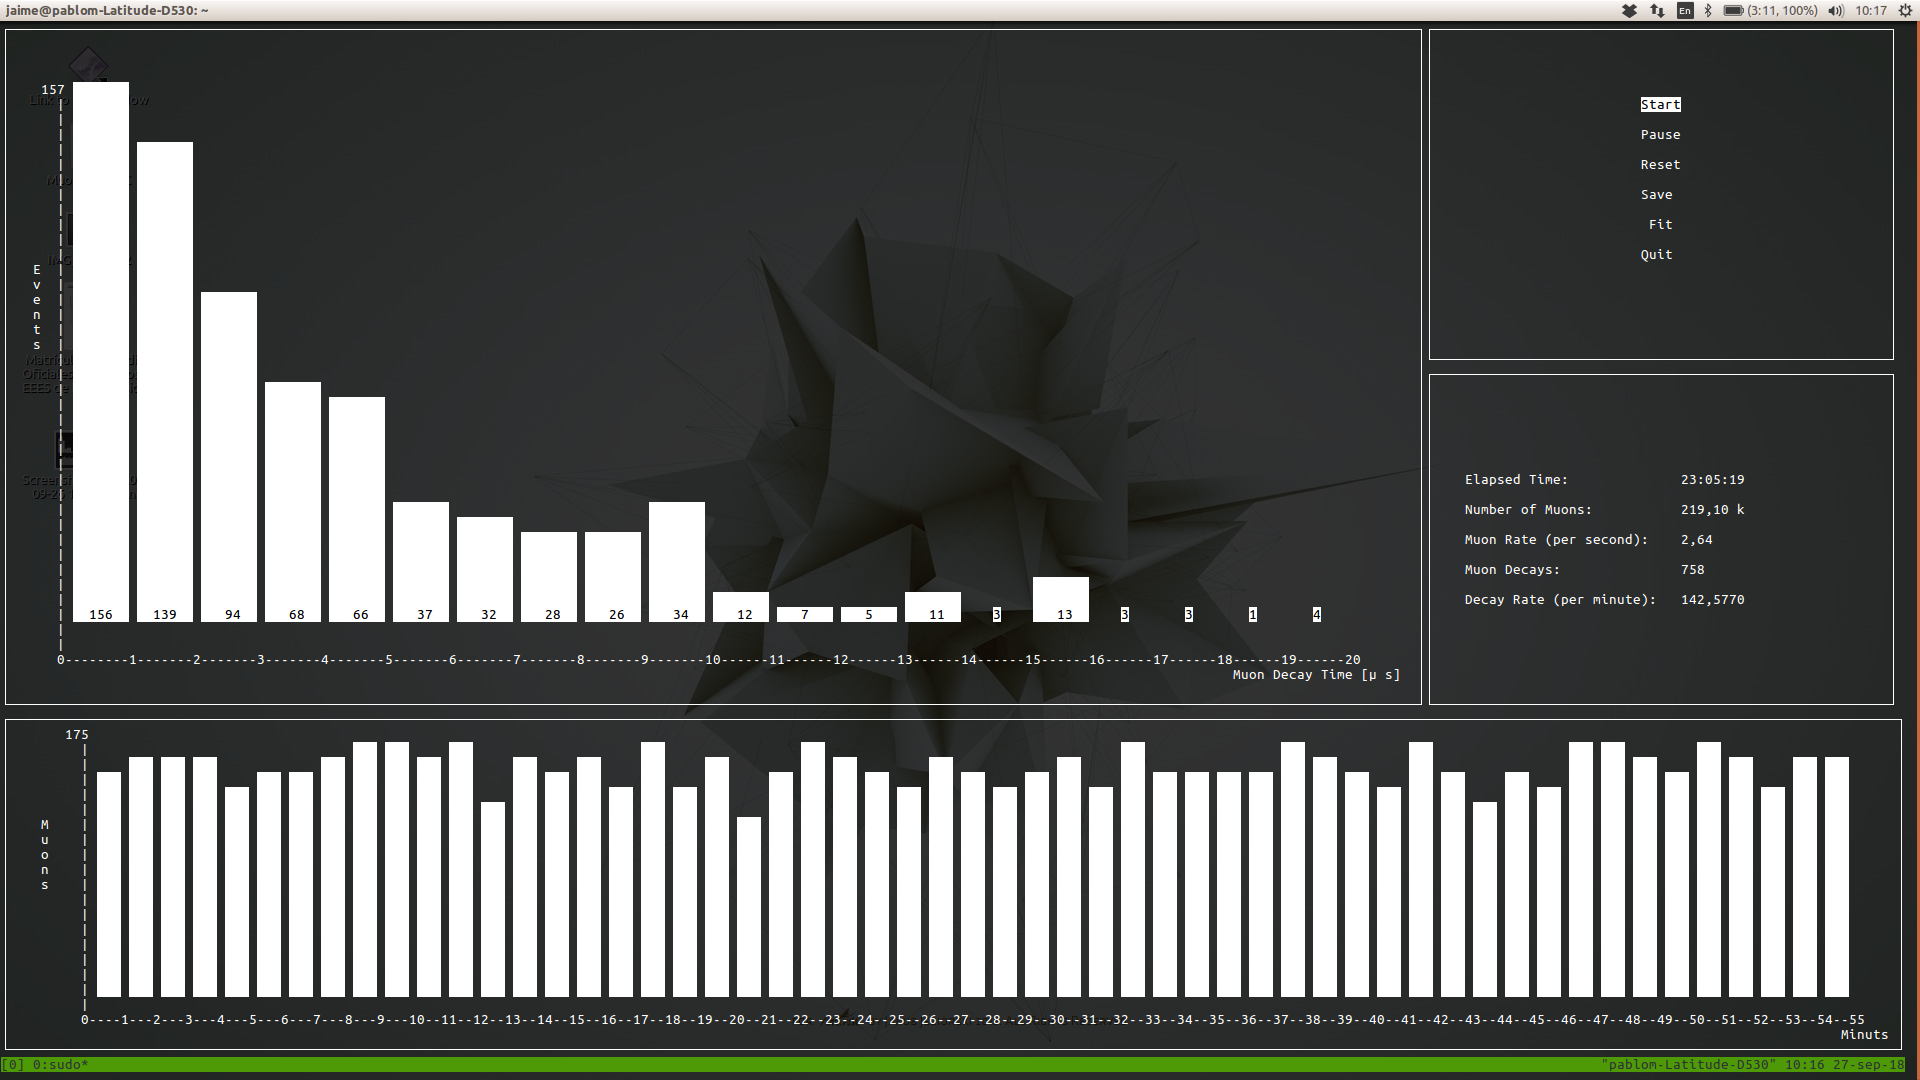
\includegraphics[scale=0.12]{Fotos/Experimento/soooPerfect.png}
                            \end{figure}
                        \end{minipage}}

                    \onslide<2->{\begin{minipage}[c]{1.4\linewidth}
                        \vspace{-2.2cm}
                        {\begin{figure}[b]
                            \centering
                            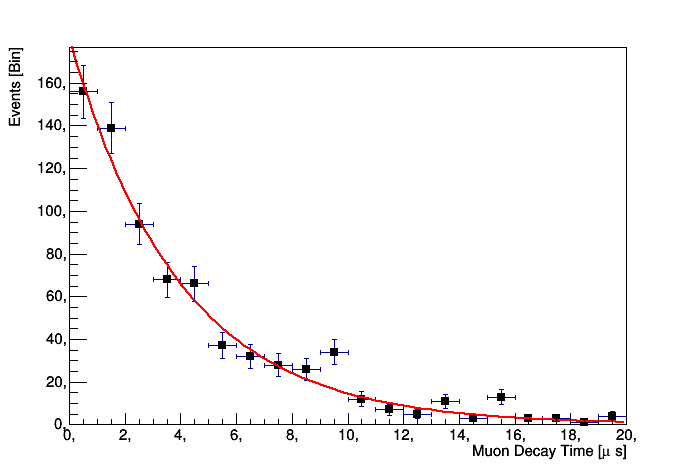
\includegraphics[scale=0.3]{Fotos/Experimento/Graph_27-9-2018.png}
                        \end{figure}}
                    \end{minipage}}

                    \onslide<2->{\begin{minipage}[c]{1.6\linewidth}
                        \vspace{-5cm}
                        {\begin{equation*}
                            P(t) = e^{-t/(\gamma \tau)}
                        \end{equation*}}
                    \end{minipage}}
                \end{frame}

                \begin{frame}
                    \frametitle{\centerline{\textbf{... y de la Dilatación Temporal}}}


                    \onslide<1->{Mediante el estudio de las relaciones entre las tasas de muones detenidos en el detector a dos alturas diferentes se puede obtener una demostración del efecto de dilatación temporal debido a la relatividad}

                    \onslide<2->{
                        \vspace{0.5cm}
                        Tiempo de tránsito en el sistema de referencia del muon con dilatación temporal
                        \begin{equation*}
                                t' \simeq \frac{mc}{\rho S_0} \int^{\gamma_1}_{\gamma_2} \frac{\textrm{d}\gamma}{\sqrt{\gamma^2 - 1}} \rightarrow S_0 = 2 MeV g^{-1} cm^{2} 
                        \end{equation*}}

                    \onslide<3->{La diferencia de altura entre los detectores producen una pérdida de energía de los muones, disminuyendo la tasa de muones detenidos en el detector a menor altura}
                 \end{frame}

                \begin{frame}
                    \frametitle{\centerline{\textbf{Niveles del Experimento}}}


                    \onslide<1->{\begin{table}[H]
                        \centering
                        \begin{tabular}{m{5.0cm} | m{3.0cm}}
                            \hline \hline
                            \multirow{1}{5.0cm}{\centering \Large \textbf{Descripción}} & \multirow{1}{3.0cm}{\centering \Large  \textbf{Público}} \\
                            & \\\hline \hline
                            Medida del tiempo de vida medio del muón mediante la ley exponencil de desintegración & Pre-Universitarios\\ \hline
                            Modelo Pre-Universitario + explicación del modelo estándar de partículas  & Primeros Cursos del grado \\ \hline
                            Primeros Cursos del grado + Dilatación temporal & Ultimos Cursos del grado \\
                            \hline
                        \end{tabular}
                    \end{table}}
                 \end{frame}

            \section{Partes a Desarrollar}

                 \begin{frame}
                    \frametitle{\centerline{\textbf{Dispositivo Compacto}}}
                    
                    \onslide<1->{\begin{minipage}[c]{1.4\linewidth}
                            %\vspace{3cm}
                            \begin{figure}[t]
                                \centering
                                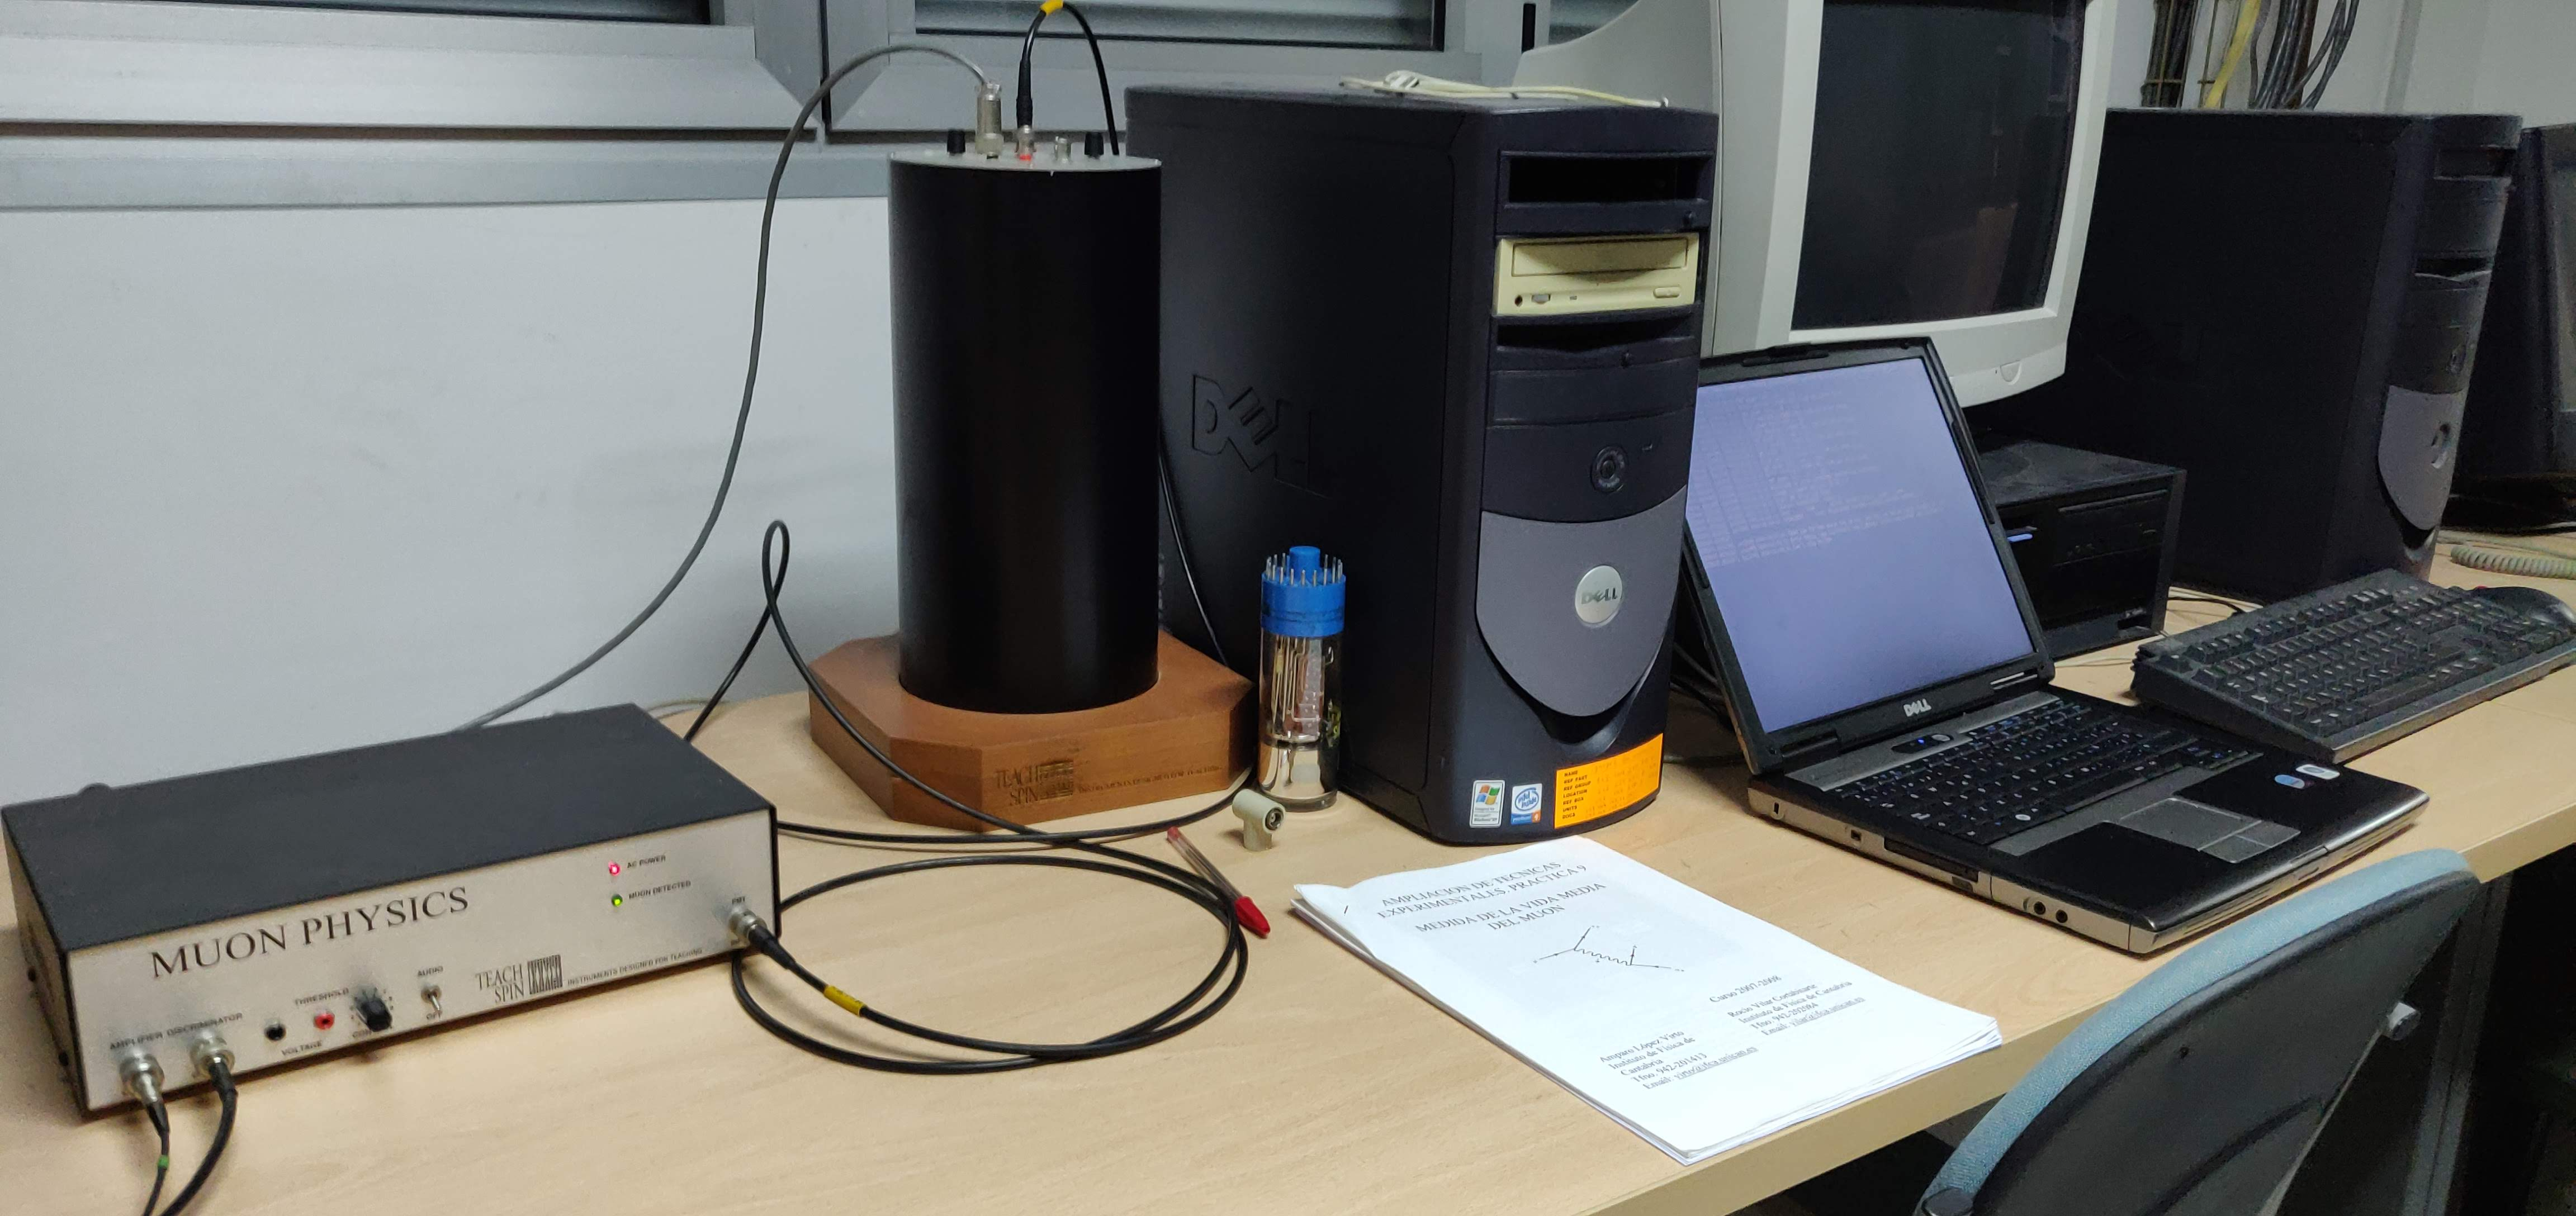
\includegraphics[scale=0.04]{Fotos/Experimento/IMG_20180927_113646.jpg}
                            \end{figure}
                        \end{minipage}}
                        \vspace{0.5cm}
                    
                    \onslide<2->{%\begin{minipage}[c]{0.3\linewidth}
                        Desarrollar un dispositivo compacto que permita su uso para la divulgación}

                    \onslide<2->{\begin{minipage}[c]{0.2\linewidth}
                        {\begin{figure}[b]
                            \centering
                            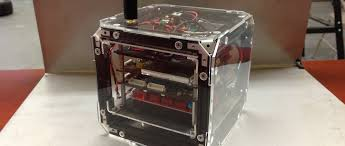
\includegraphics[scale=0.4]{Fotos/download(1).jpeg}
                        \end{figure}}
                    \end{minipage}}
                 \end{frame}

                 \begin{frame}
                    \frametitle{\centerline{\textbf{Dispositivo Autosuficiente}}}
                    
                    \onslide<1->{\begin{minipage}[c]{1.4\linewidth}
                            %\vspace{3cm}
                            \begin{figure}[t]
                                \centering
                                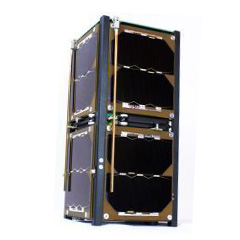
\includegraphics[scale=0.4]{Fotos/NanoRacks-ArduSat-2.jpg}
                            \end{figure}
                        \end{minipage}}
                        \vspace{-0.5cm}
                    
                    \onslide<1->{%\begin{minipage}[c]{0.3\linewidth}
                        El dispositivo estará diseñado para su funcionamiento de forma remota en lugares de gran altitud y contará con:

                        \begin{itemize}
                            \item Paneles Solares
                            \item Sistema de comunicación UHF \textit{Half Duplex}
                        \end{itemize}}

                    \onslide<2->{ Los dispositivos estarán conectados a una red controlada mediante una página web a la que se pondrá conectar durante las jornadas de divulgación o realización del experimento}
                 \end{frame}

            \section{Realización}
                  \begin{frame}
                    \frametitle{\centerline{\textbf{Realización del Proyecto}}}
                    
                    \onslide<1->{El proyecto tiene la fecha de inicio en el 3 de Junio de 2019 y se prevee poder concluirlo para el 3 de Junio de 2022}
                        \vspace{0.5cm}
                    
                    \onslide<2->{\begin{table}[H]
                            \centering
                            \footnotesize
                            \begin{tabular}{ c c c c }
                                \hline
                                \centering
                                    Work Package    & Nombre del WP     & Comienzo del WP   & Fin del WP \\ \hline
                                    \hline
                                    WP1             & Coordinación      &  06/2019        & 06/2022 \\ \hline
                                    WP2             & Investigación     &  06/2019        & 09/2019 \\ \hline
                                    WP3             & Difusión          &  09/2019        & 06/2022 \\ \hline
                                    WP4             & Dispositivos      &  09/2019        & 11/2020 \\ \hline
                                    WP5             & Muon Web          &  04/2020        & 01/2021 \\ \hline
                            \end{tabular}
                        \end{table}}

                    \onslide<3->{\begin{figure}[H]
                        \centering
                        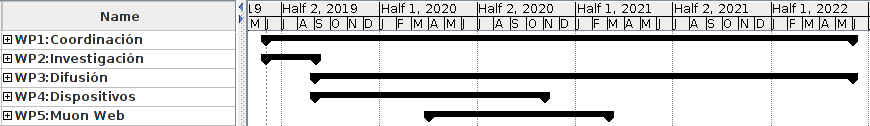
\includegraphics[scale=0.3]{Fotos/GanttWP.png}
                    \end{figure}}
                 \end{frame}

            \section{Riesgos}

                \begin{frame}
                    \frametitle{\centerline{\textbf{Riesgos}}}


                    \onslide<1->{\begin{table}[H]
                        \centering
                        \tiny
                        \begin{tabular}{m{3.0cm} m{1.0cm} m{1.0cm} m{3.0cm}}
                            \hline
                            \multicolumn{1}{m{3.0cm}}{\centering \textbf{Descripción del Riesgo}} &  
                            \multicolumn{1}{m{1.5cm}}{\centering \textbf{Probabilidad}} &
                            \multicolumn{1}{m{1.4cm}}{\centering \textbf{WP afectados}} &
                            \multicolumn{1}{m{3.cm}}{\centering \textbf{Propuesta para mitigarlo}}  \\ \hline
                            \hline
                            Fallo en el sistema de autoavastecimiento energético del dispositivo experimental & Media & WP3, WP4 & Se buscaría más apoyo de centros que acogiesen los dispositivos \\ \hline
                            Alto coste de producción de los dispositivos & Bajo & WP1, WP4 & Se buscaría abaratar el dispositivo disminuyendo sus prestaciones, además de la busqueda de nuevas fuentes de financiación \\ \hline
                            Falta de interés por parte de Intitutos & Bajo & WP3 & Se buscaría una nueva via para llegar a los jovenes interesados en las jornadas \\ \hline
                            Falta de interés por parte de los alumnos & Bajo & WP3 & Cambiaar el contenido de las jornadas para hacerlas más atractivas para el alumnado \\ \hline      
                        \end{tabular}
                    \end{table}}
                 \end{frame}

    %----------------------------------------------------------------------------
    %     BIBLIOGRAPHY
    %----------------------------------------------------------------------------

        \bibliographystyle{unsrt}
        \bibliography{biblio}

    \end{document} 